\chapter{Intrinsic experiments}
\label{cha:experiments}

% \section{Similarity and relatedness of words}
% \label{sec:lexical}

% Table~\ref{tab:parameters} lists parameters and their values. As the source corpus we use the concatenation of Wackypedia and ukWaC \cite{ukwac} with a symmetric 5-word window \cite{milajevs-EtAl:2014:EMNLP2014}; our evaluation metric is the correlation with human judgements as is standard with SimLex \cite{hill2014simlex}. We derive our parameter selection heuristics by greedily selecting parameters (\texttt{cds}, \texttt{neg}) that lead to the highest average performance for each combination of frequency weighting, PMI variant and dimensionality $D$. Figures~\ref{fig:interaction-cds} and \ref{fig:interaction-neg} show the interaction of \texttt{cds} and \texttt{neg} with other parameters. We also vary the similarity measure (cosine and correlation  \cite{kiela-clark:2014:CVSC}), but do not report results here due to space limits.

% % \begin{wraptable}[13]{O}{0.5\textwidth}
\begin{table}
  % \vspace{-2em}
  \centering
  \small
  \begin{tabular}{lcl}
    \toprule
    Parameter           & Abbreviation   & Values \\
    \midrule
    Dimensionality      & $D$            & 1K, 2K, 3K, 5K, 10K, 20K, 30K, 40K, 50K \\
    Discriminativeness  & \texttt{discr} & PMI, CPMI, SPMI, \textbf{SCPMI} \\
    Frequency weighting & \texttt{freq}  & $1$, $n$, $\boldsymbol{\log n}$ \\
    Shifting            & \texttt{neg}   & \textbf{0.2}, \textbf{0.5}, \textbf{0.7}, 1, 1.4, 2, 5, 7 \\
    Context distribution smoothing       & \texttt{cds} & \textbf{\textit{global}}, 1, 0.75 \\
    Similarity          &                & Cosine, Correlation and Inner product \\
    \addlinespace
    Window size         &                & 5 from both sides                     \\
    Corpus              &                & Concatenation of ukWaC and Wackypedia \\
    \bottomrule
  \end{tabular}
  \caption{Model parameters and their values used in the experiments. To our knowledge, values are bold have not been used previously.}
\label{tab:parameters}
\end{table}

%%% Local Variables:
%%% mode: latex
%%% TeX-master: "../thesis"
%%% End:




% \clearpage
% \KOMAoptions{paper=A3}
% % \addtolength{\textwidth}{1.35\textwidth}
% \recalctypearea

\newgeometry{margin=1.5cm}

\begin{landscape}
\thispagestyle{empty} %% Remove header and footer.

\begin{figure}
  \centering

  \begin{subfigure}[t]{0.49\textwidth}
    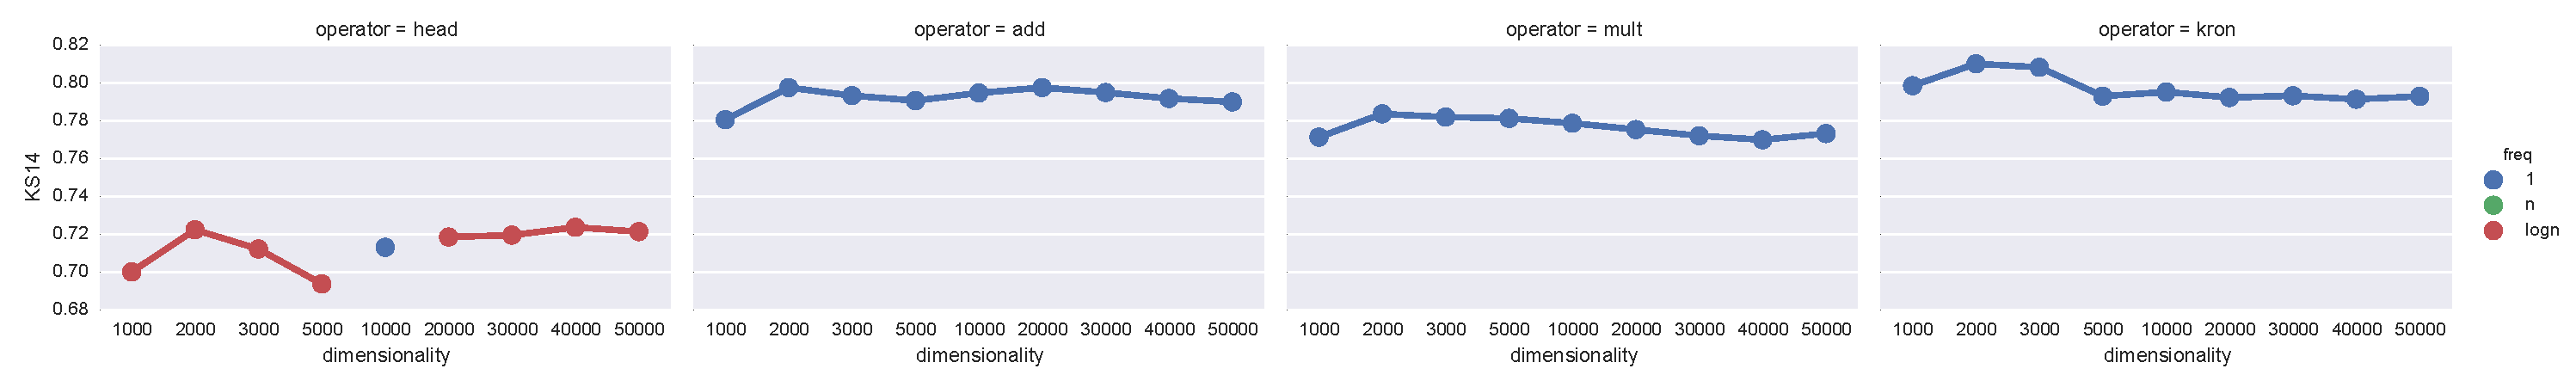
\includegraphics[width=\textwidth]{supplement/figures/KS14-max_-selection-freq}
    \caption{Max. Freq.}
    \label{fig:}
  \end{subfigure}
  \begin{subfigure}[t]{0.49\textwidth}
    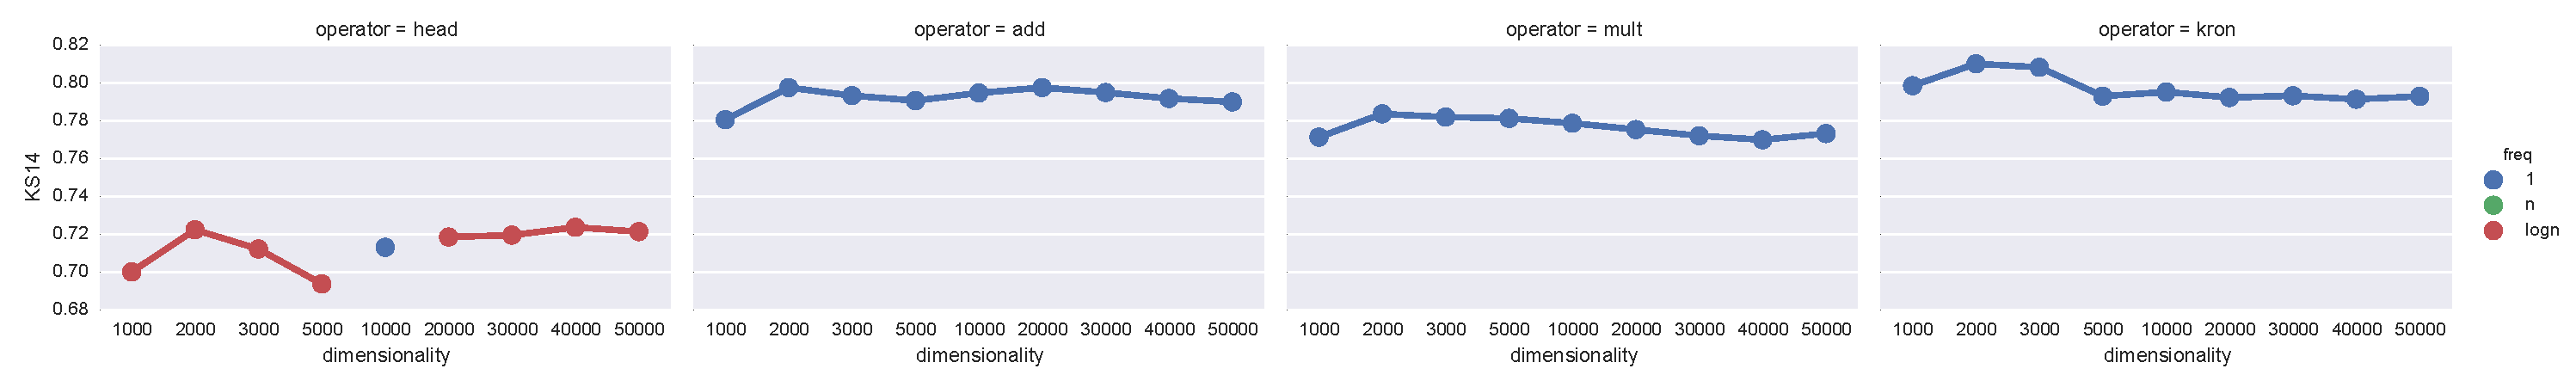
\includegraphics[width=\textwidth]{supplement/figures/KS14-cross_validation-selection-freq}
    \caption{CV. Freq.}
    \label{fig:}
  \end{subfigure}
  \begin{subfigure}[t]{0.49\textwidth}
    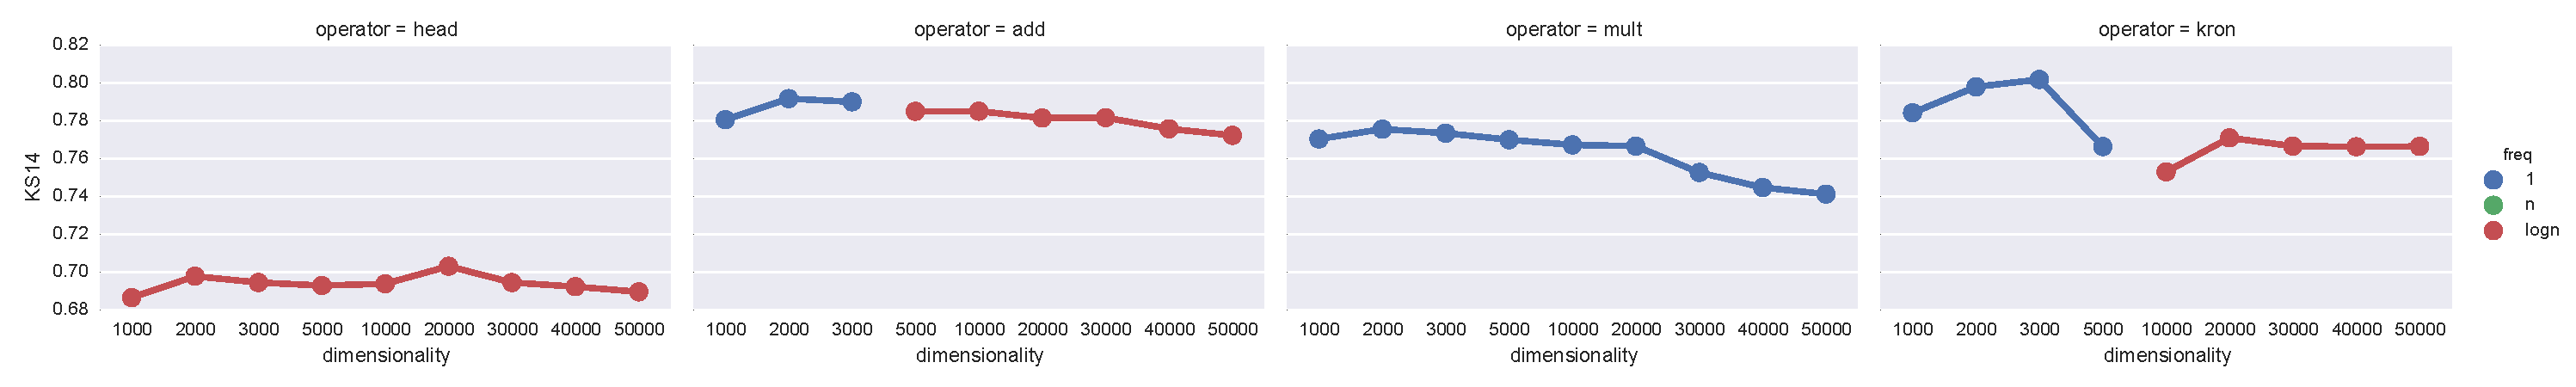
\includegraphics[width=\textwidth]{supplement/figures/KS14-heuristics-selection-freq}
    \caption{H. Freq.}
    \label{fig:}
  \end{subfigure}

  \begin{subfigure}[t]{0.49\textwidth}
    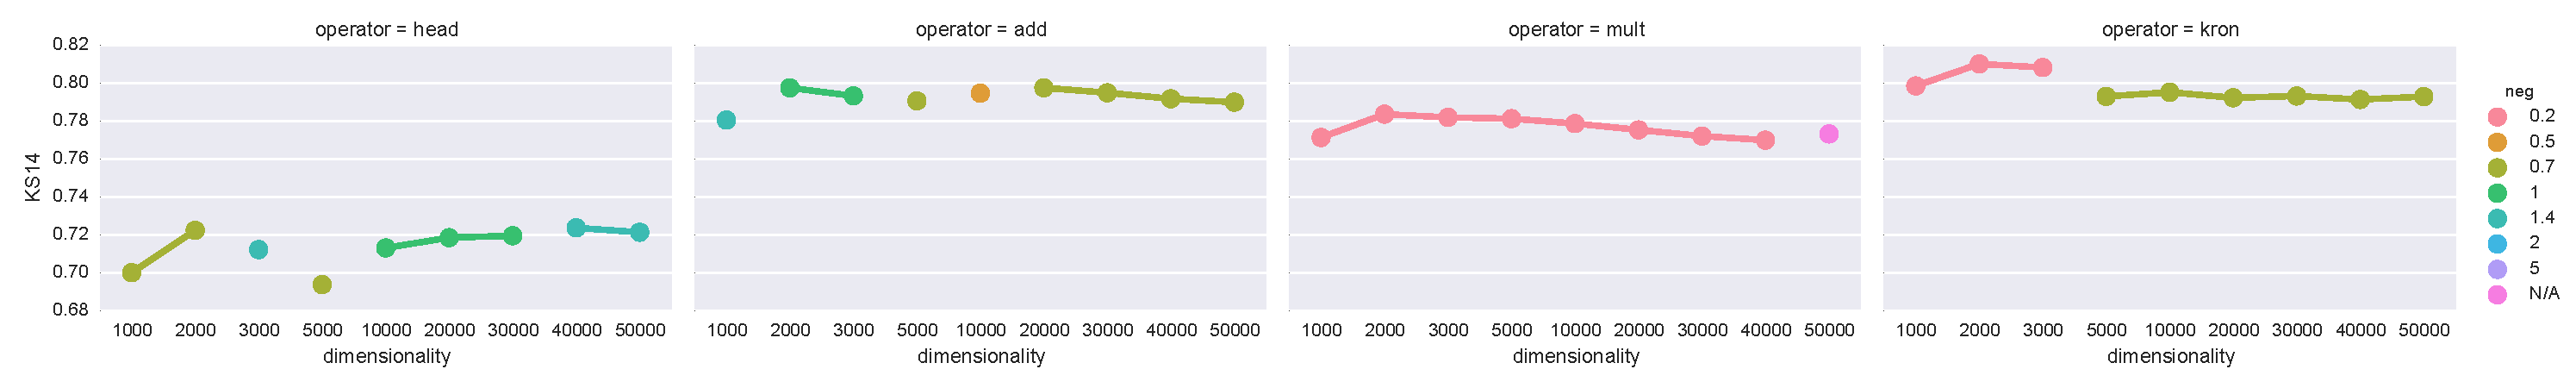
\includegraphics[width=\textwidth]{supplement/figures/KS14-max_-selection-neg}
    \caption{Max. Neg.}
    \label{fig:}
  \end{subfigure}
  \begin{subfigure}[t]{0.49\textwidth}
    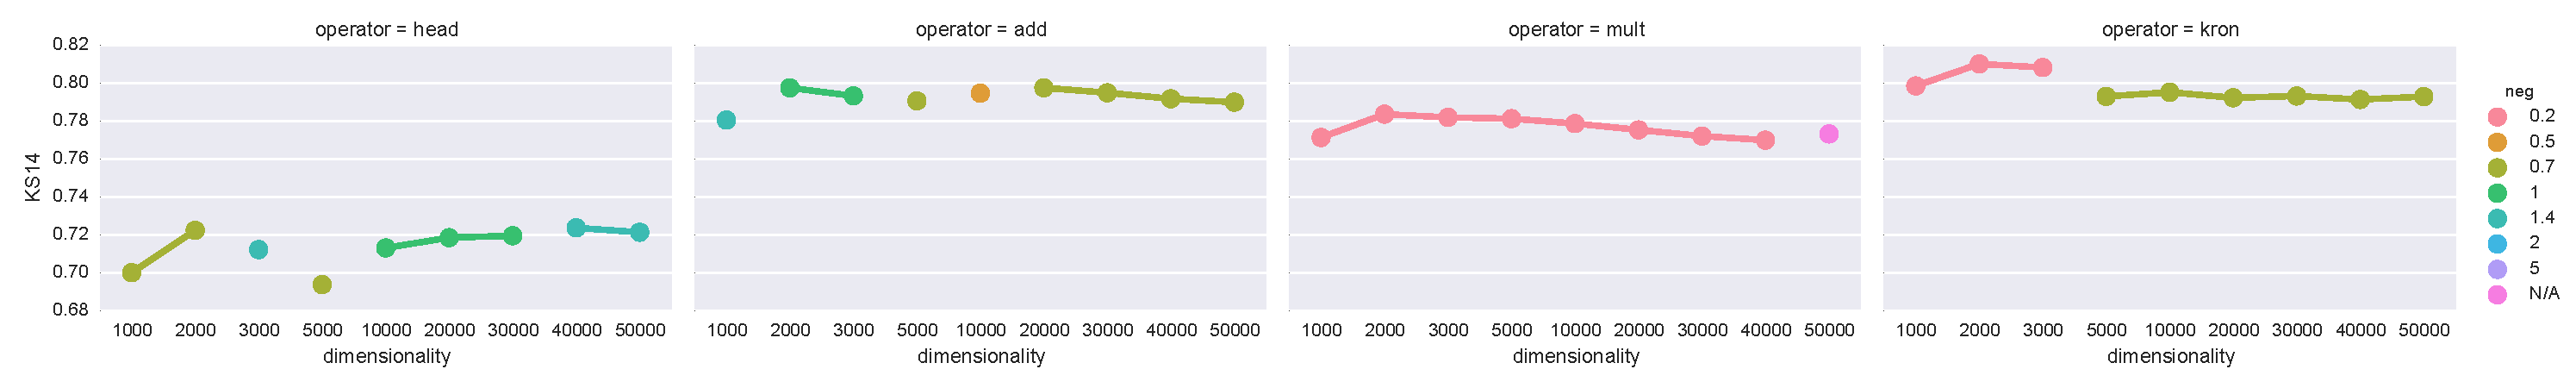
\includegraphics[width=\textwidth]{supplement/figures/KS14-cross_validation-selection-neg}
    \caption{CV. Neg.}
    \label{fig:}
  \end{subfigure}
  \begin{subfigure}[t]{0.49\textwidth}
    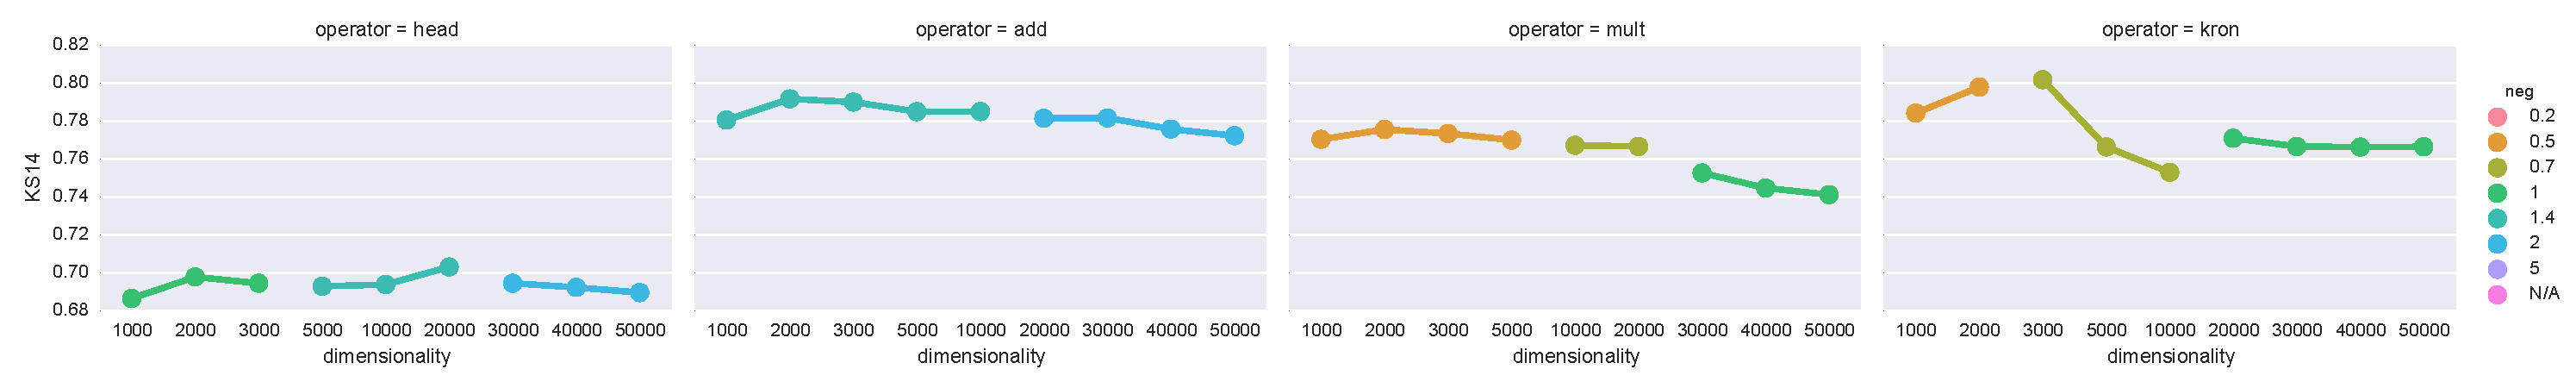
\includegraphics[width=\textwidth]{supplement/figures/KS14-heuristics-selection-neg}
    \caption{H. Neg.}
    \label{fig:}
  \end{subfigure}

  \begin{subfigure}[t]{0.49\textwidth}
    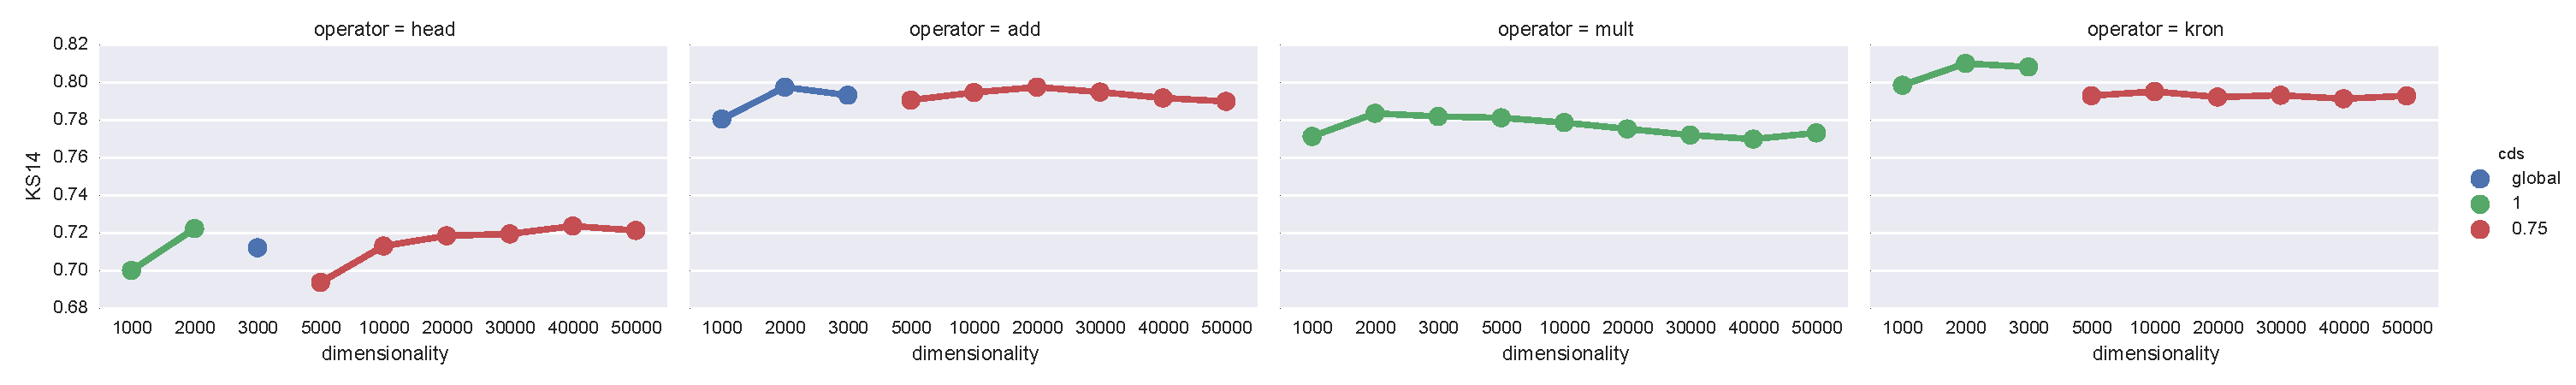
\includegraphics[width=\textwidth]{supplement/figures/KS14-max_-selection-cds}
    \caption{Max. CDS.}
    \label{fig:}
  \end{subfigure}
  \begin{subfigure}[t]{0.49\textwidth}
    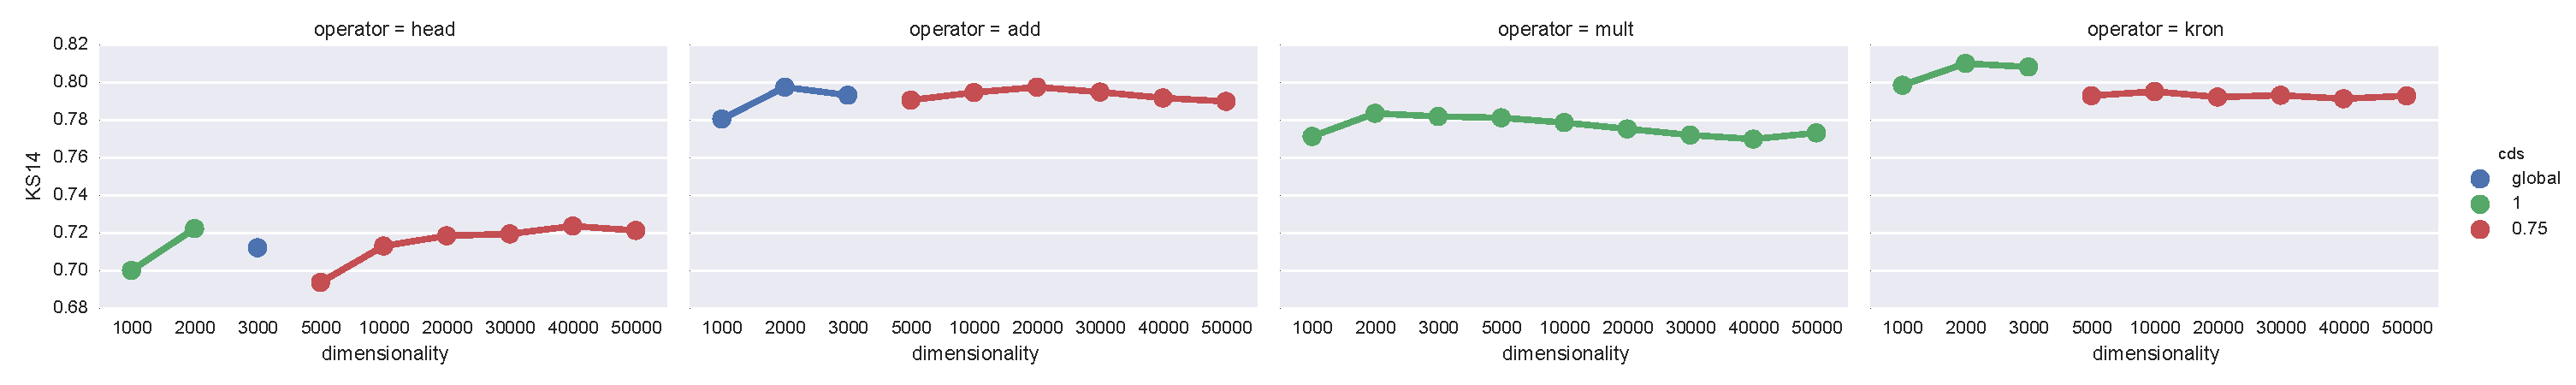
\includegraphics[width=\textwidth]{supplement/figures/KS14-cross_validation-selection-cds}
    \caption{CV. CDS.}
    \label{fig:}
  \end{subfigure}
  \begin{subfigure}[t]{0.49\textwidth}
    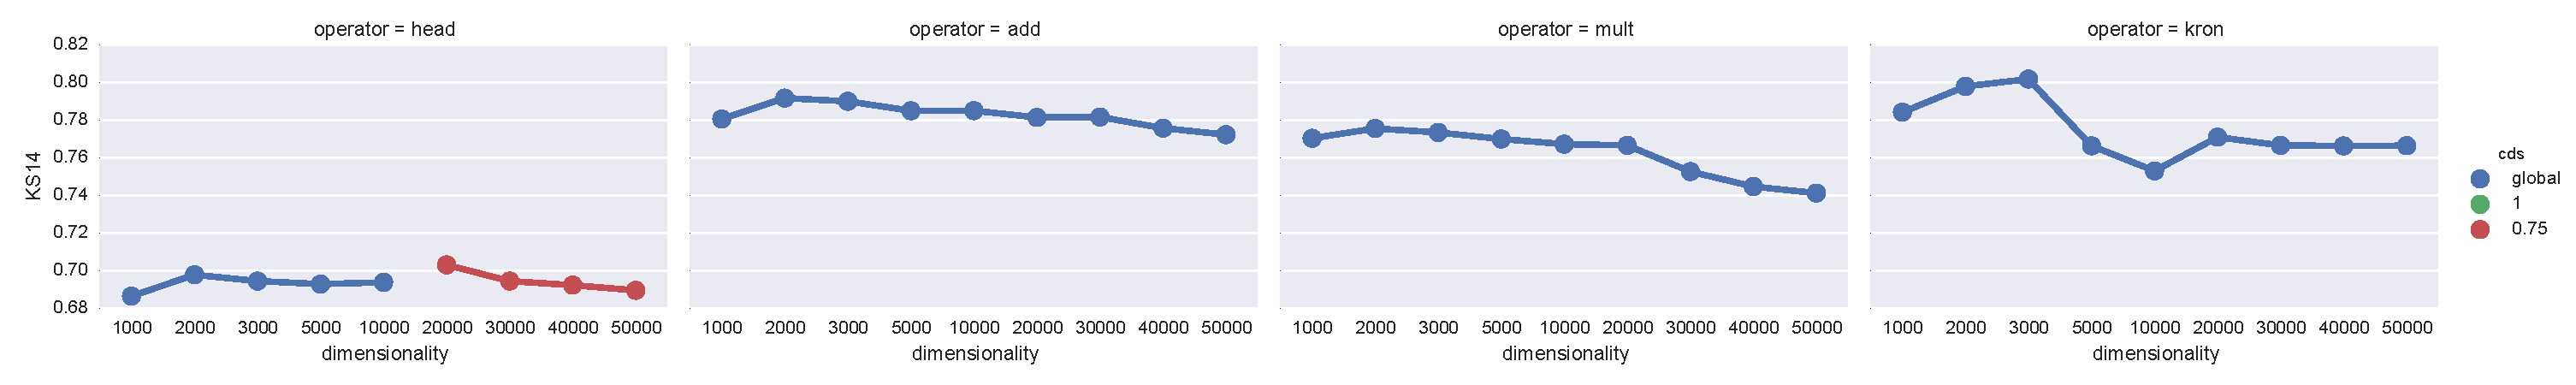
\includegraphics[width=\textwidth]{supplement/figures/KS14-heuristics-selection-cds}
    \caption{H. CDS.}
    \label{fig:}
  \end{subfigure}

  \begin{subfigure}[t]{0.49\textwidth}
    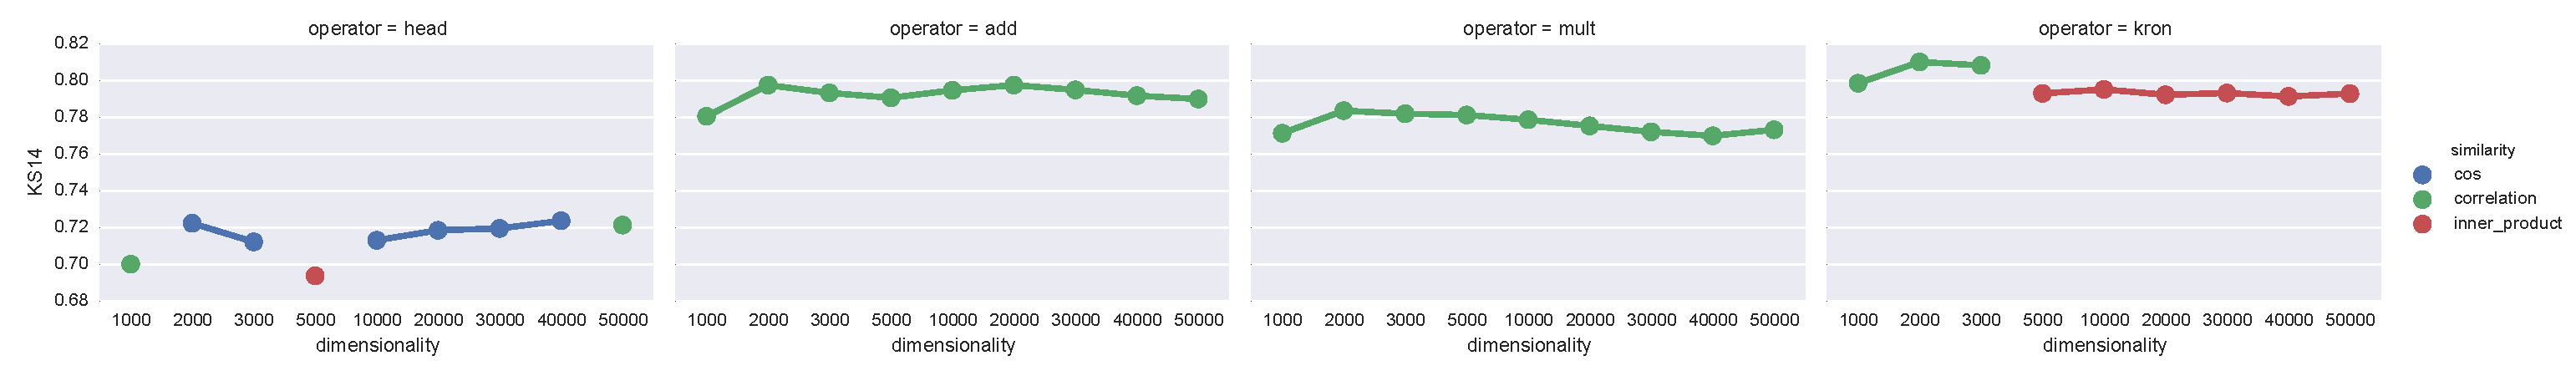
\includegraphics[width=\textwidth]{supplement/figures/KS14-max_-selection-similarity}
    \caption{Max. Sim.}
    \label{fig:}
  \end{subfigure}
  \begin{subfigure}[t]{0.49\textwidth}
    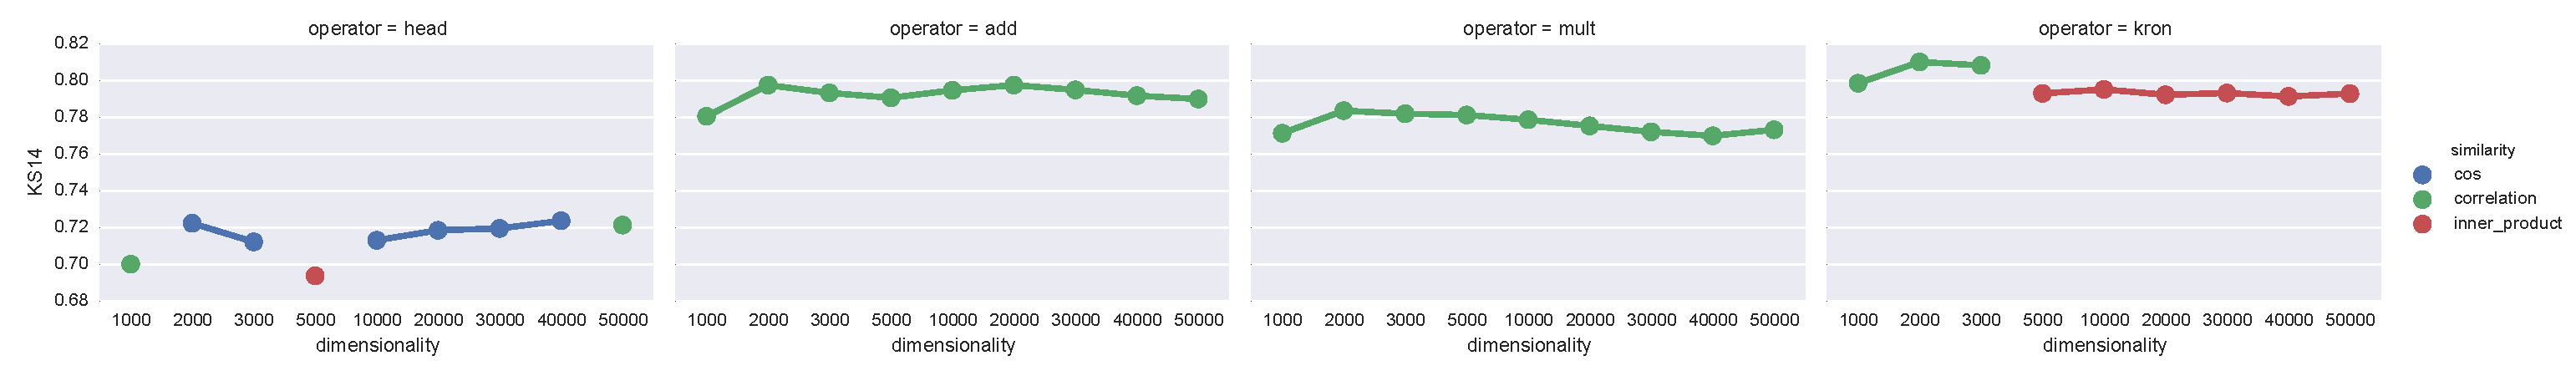
\includegraphics[width=\textwidth]{supplement/figures/KS14-cross_validation-selection-similarity}
    \caption{CV. Sim.}
    \label{fig:}
  \end{subfigure}
  \begin{subfigure}[t]{0.49\textwidth}
    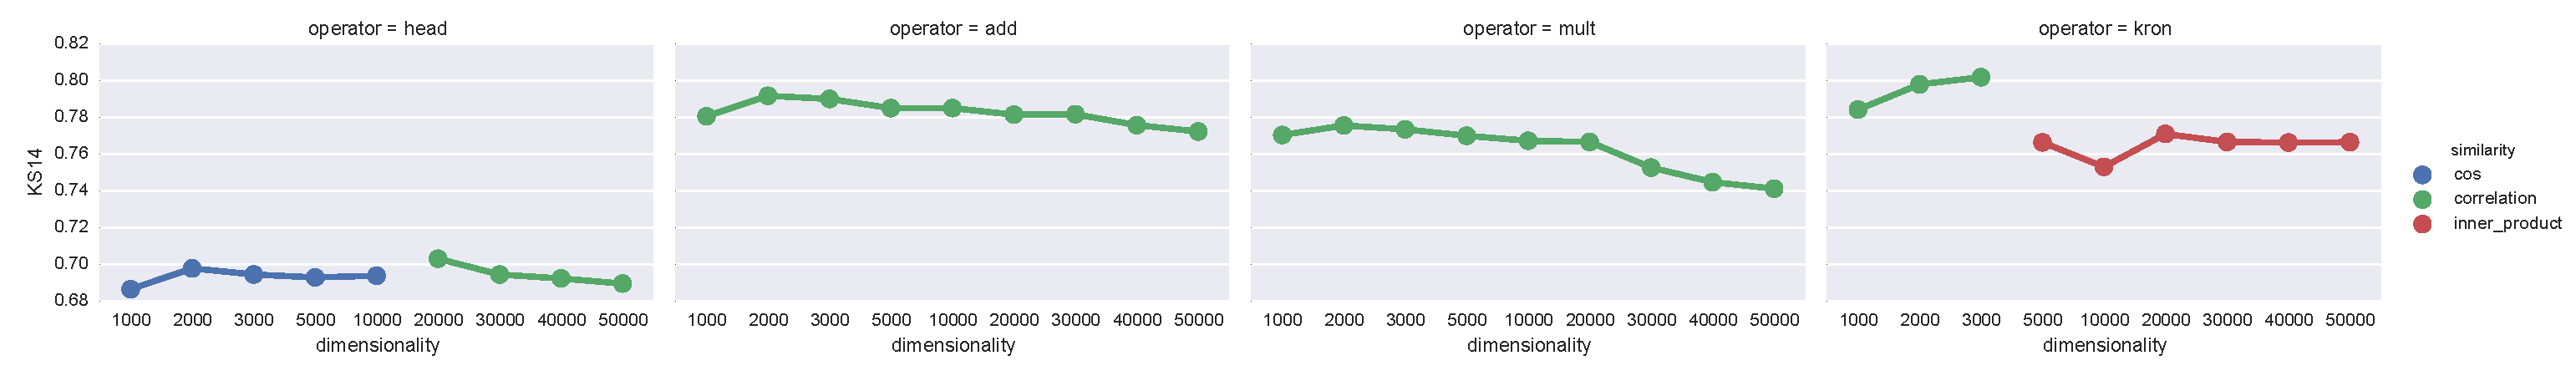
\includegraphics[width=\textwidth]{supplement/figures/KS14-heuristics-selection-similarity}
    \caption{H. Sim.}
    \label{fig:}
  \end{subfigure}

  \begin{subfigure}[t]{0.49\textwidth}
    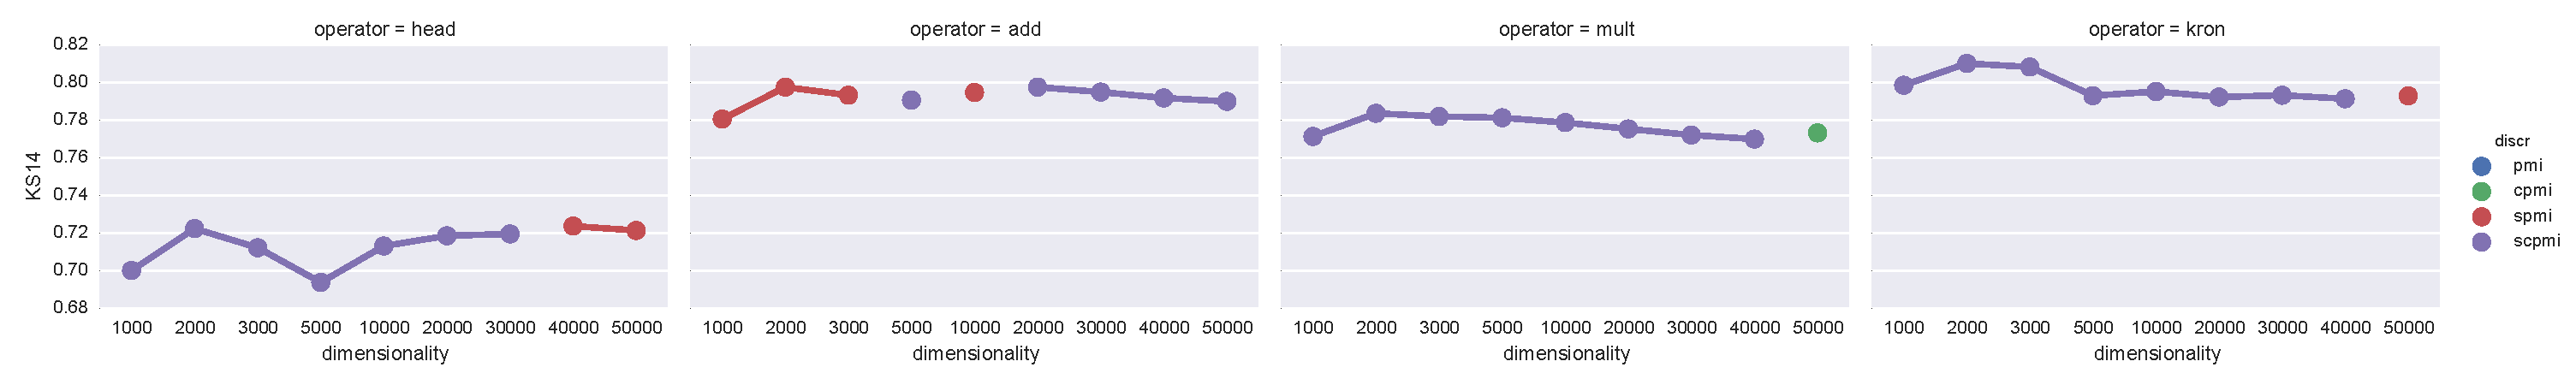
\includegraphics[width=\textwidth]{supplement/figures/KS14-max_-selection-discr}
    \caption{Max. Discr.}
    \label{fig:}
  \end{subfigure}
  \begin{subfigure}[t]{0.49\textwidth}
    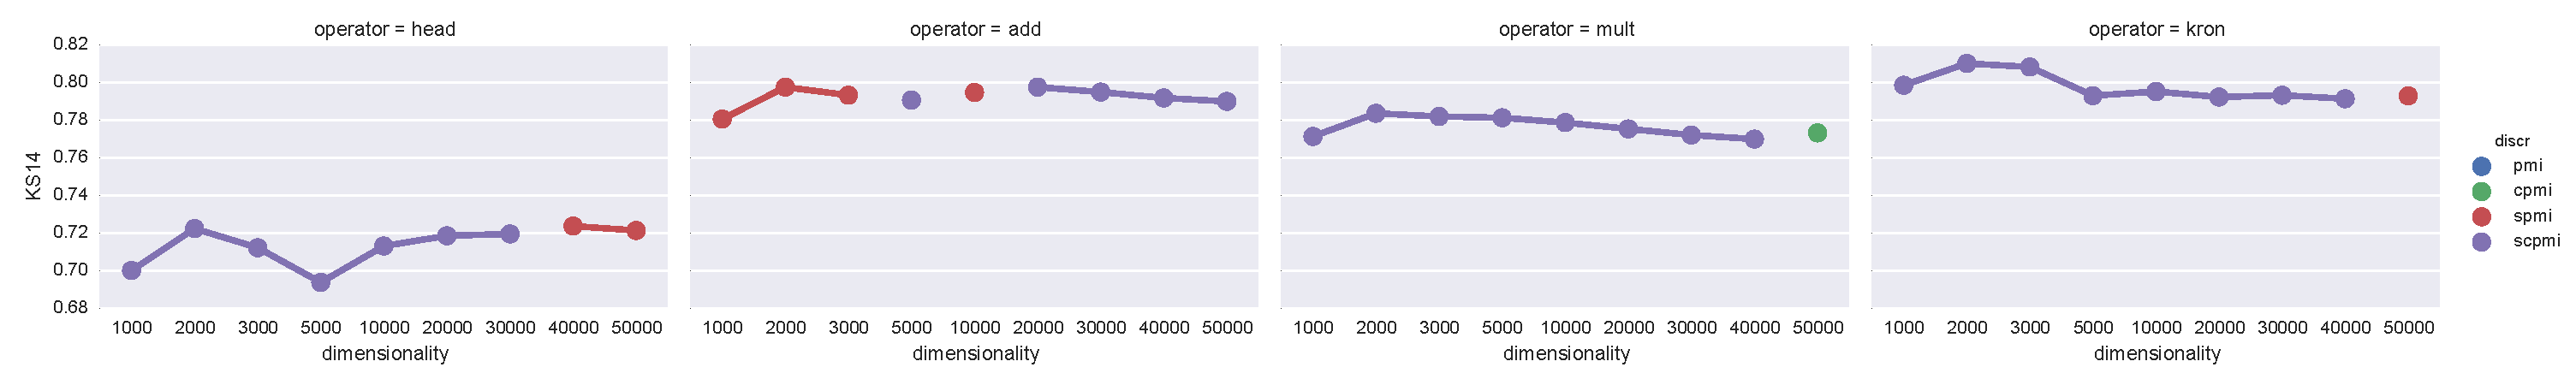
\includegraphics[width=\textwidth]{supplement/figures/KS14-cross_validation-selection-discr}
    \caption{CV. Discr.}
    \label{fig:}
  \end{subfigure}
  \begin{subfigure}[t]{0.49\textwidth}
    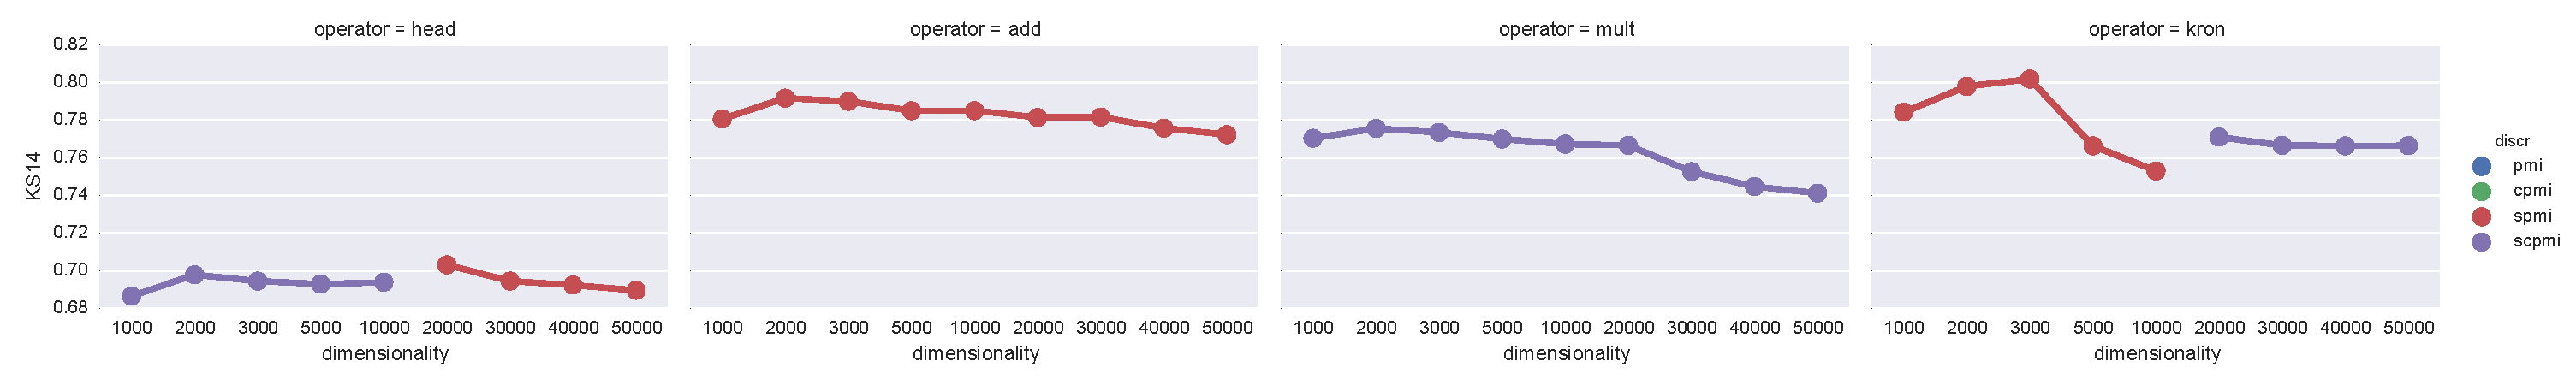
\includegraphics[width=\textwidth]{supplement/figures/KS14-heuristics-selection-discr}
    \caption{H. Discr.}
    \label{fig:}
  \end{subfigure}


  \caption{KS14 selection.}
  \label{fig:selection_ks14}
\end{figure}

\end{landscape}

\restoregeometry

% \clearpage
% \KOMAoptions{paper=A4,pagesize}
% \recalctypearea

% \clearpage
% \KOMAoptions{paper=A3}
% % \addtolength{\textwidth}{1.35\textwidth}
% \recalctypearea

\newgeometry{margin=1.5cm}

\begin{landscape}
% \thispagestyle{empty} %% Remove header and footer.

\begin{figure}
  \centering

  \begin{subfigure}[t]{0.7\textwidth}
    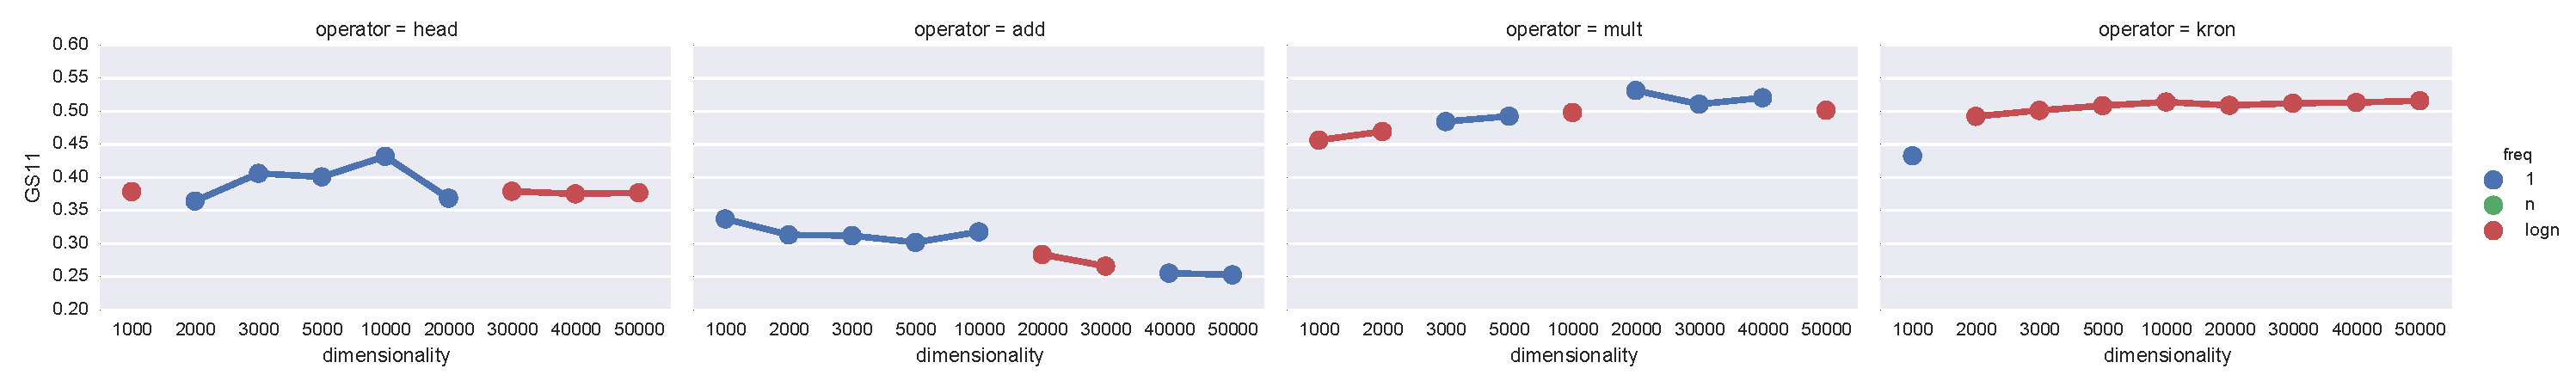
\includegraphics[width=\textwidth]{supplement/figures/GS11-max_-selection-freq}
    \caption{Max. Freq.}
    \label{fig:}
  \end{subfigure}
  % \begin{subfigure}[t]{0.7\textwidth}
  %   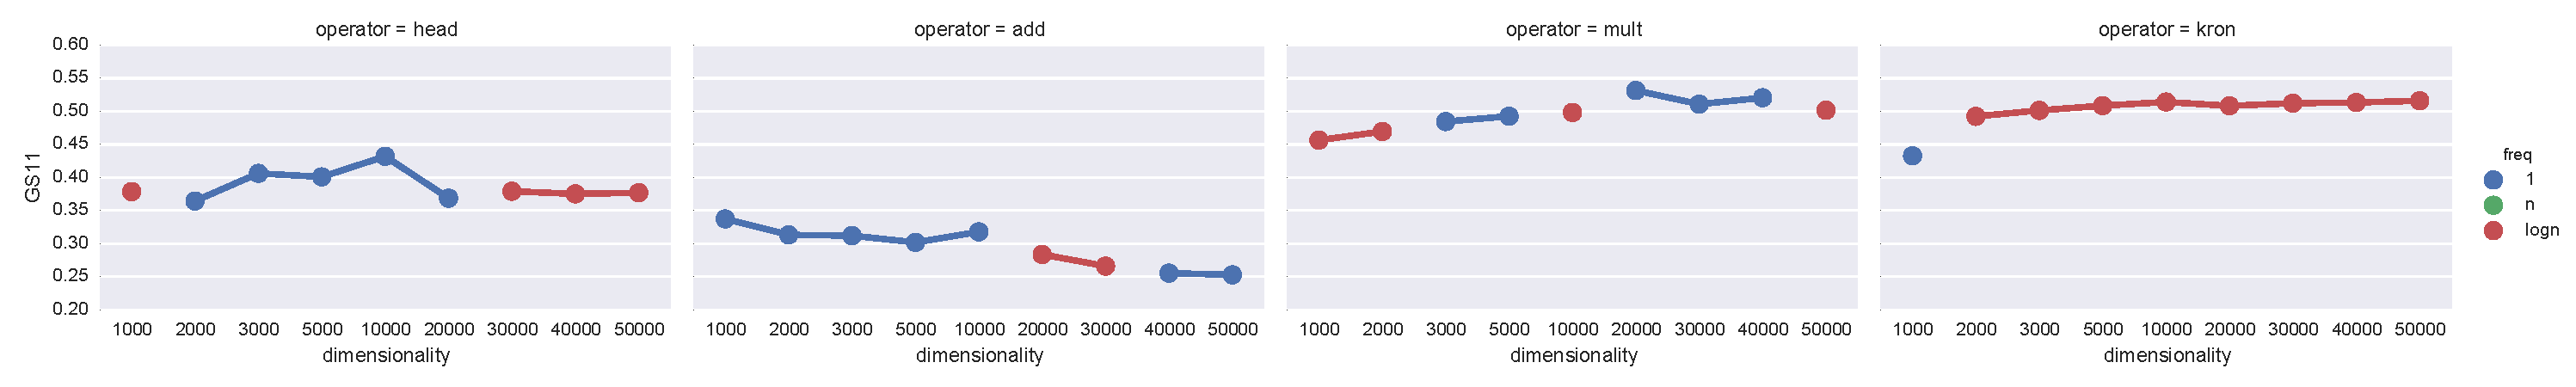
\includegraphics[width=\textwidth]{supplement/figures/GS11-cross_validation-selection-freq}
  %   \caption{CV. Freq.}
  %   \label{fig:}
  % \end{subfigure}
  \begin{subfigure}[t]{0.7\textwidth}
    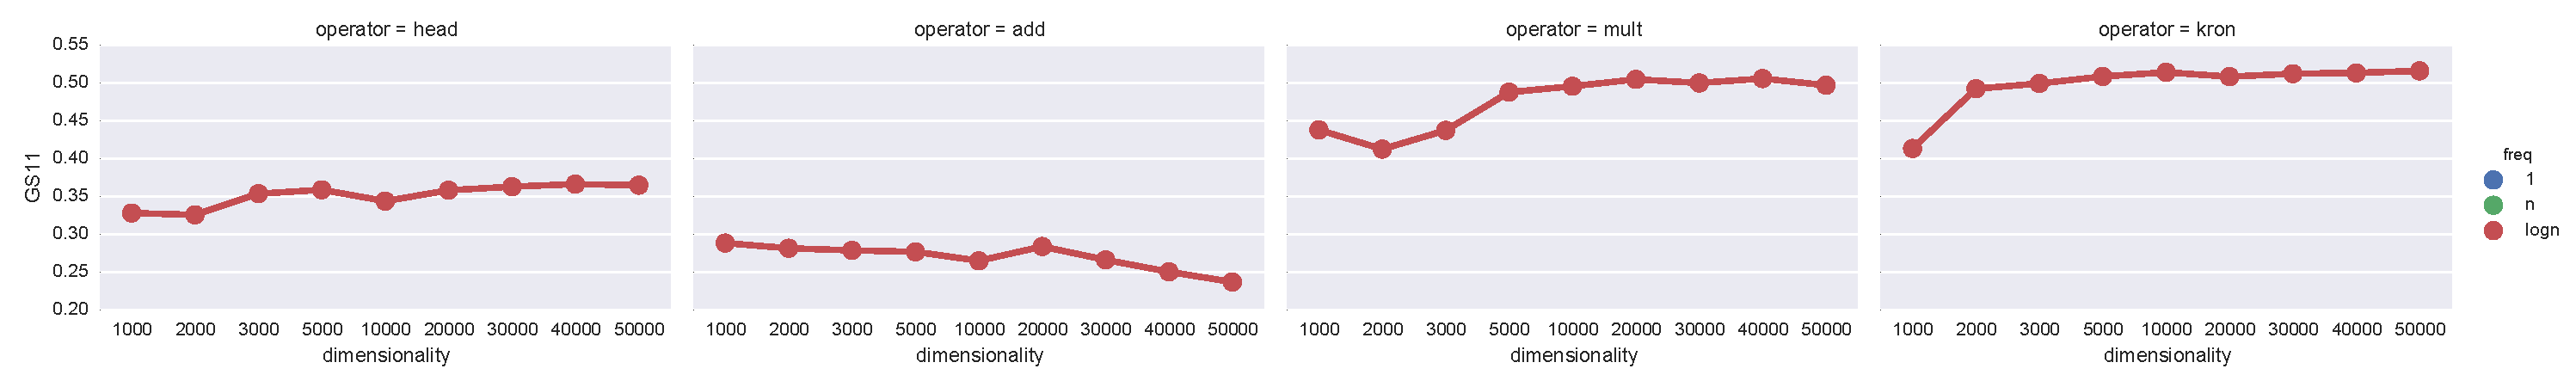
\includegraphics[width=\textwidth]{supplement/figures/GS11-heuristics-selection-freq}
    \caption{H. Freq.}
    \label{fig:}
  \end{subfigure}

  \begin{subfigure}[t]{0.7\textwidth}
    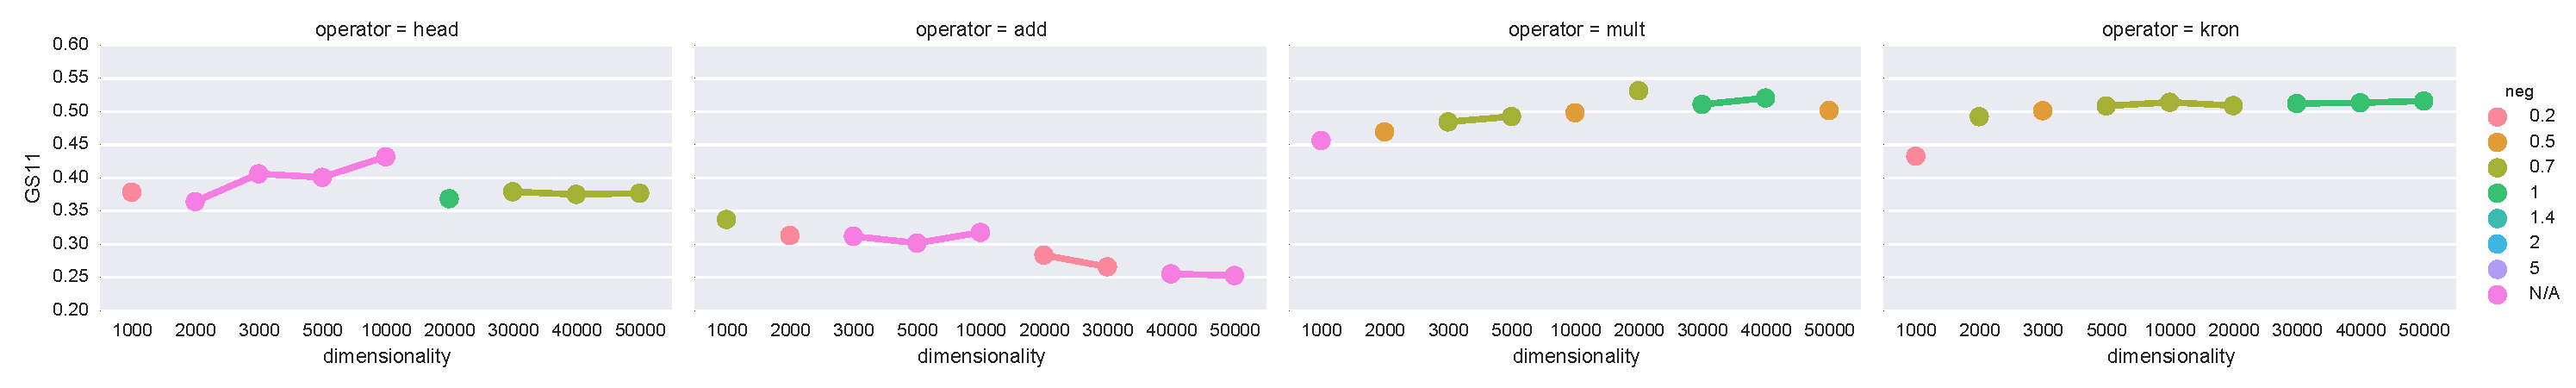
\includegraphics[width=\textwidth]{supplement/figures/GS11-max_-selection-neg}
    \caption{Max. Neg.}
    \label{fig:}
  \end{subfigure}
  % \begin{subfigure}[t]{0.7\textwidth}
  %   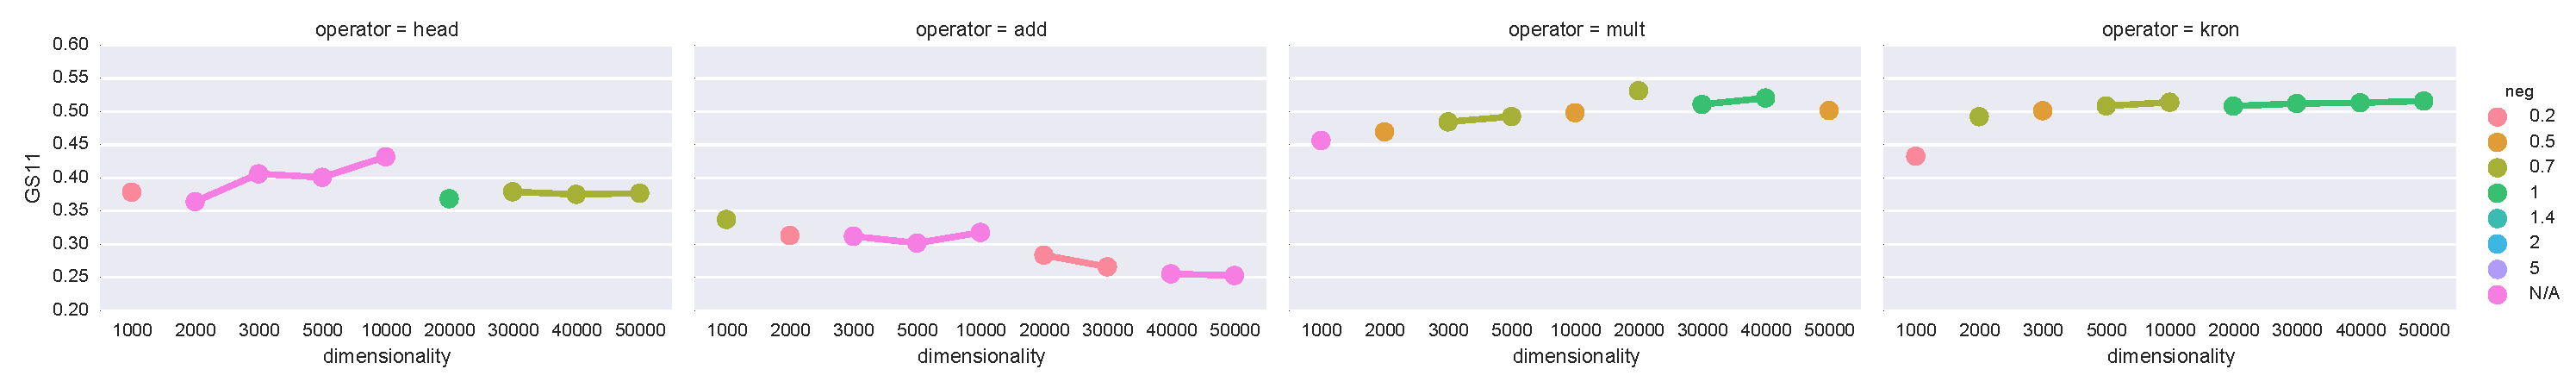
\includegraphics[width=\textwidth]{supplement/figures/GS11-cross_validation-selection-neg}
  %   \caption{CV. Neg.}
  %   \label{fig:}
  % \end{subfigure}
  \begin{subfigure}[t]{0.7\textwidth}
    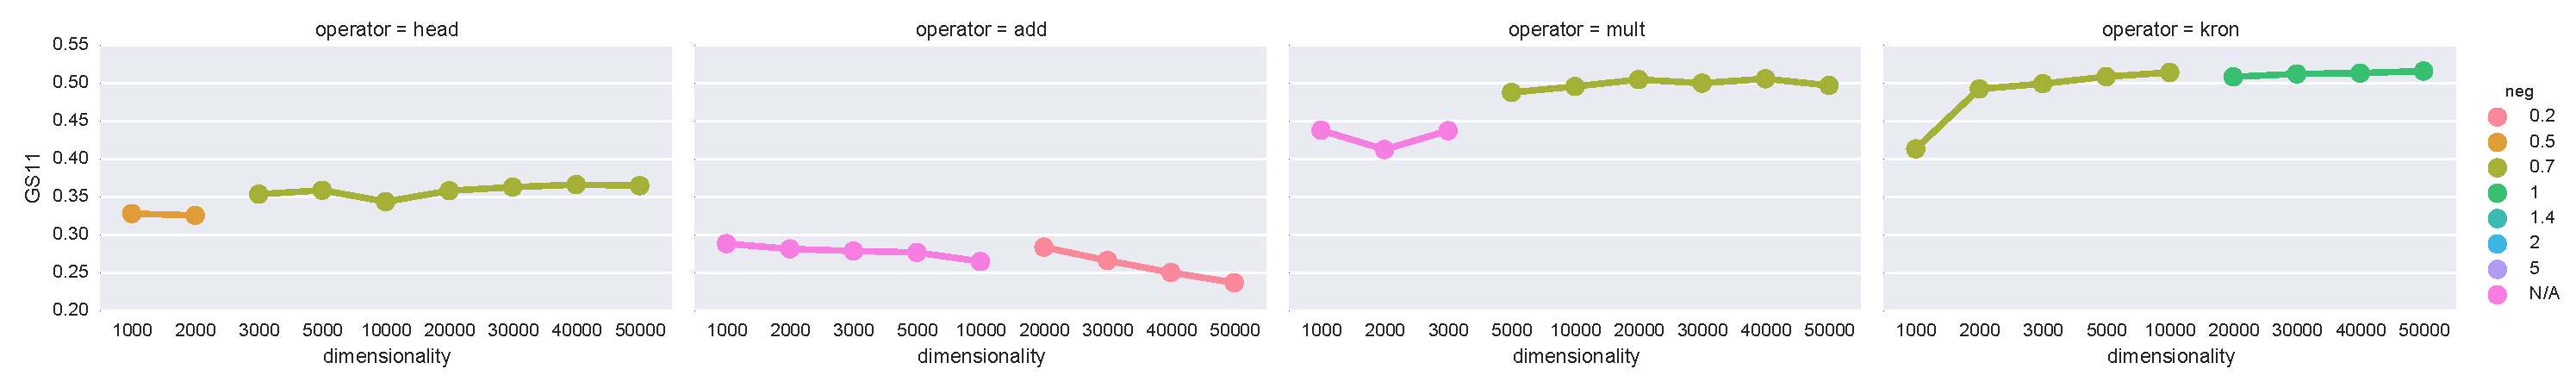
\includegraphics[width=\textwidth]{supplement/figures/GS11-heuristics-selection-neg}
    \caption{H. Neg.}
    \label{fig:}
  \end{subfigure}

  \begin{subfigure}[t]{0.7\textwidth}
    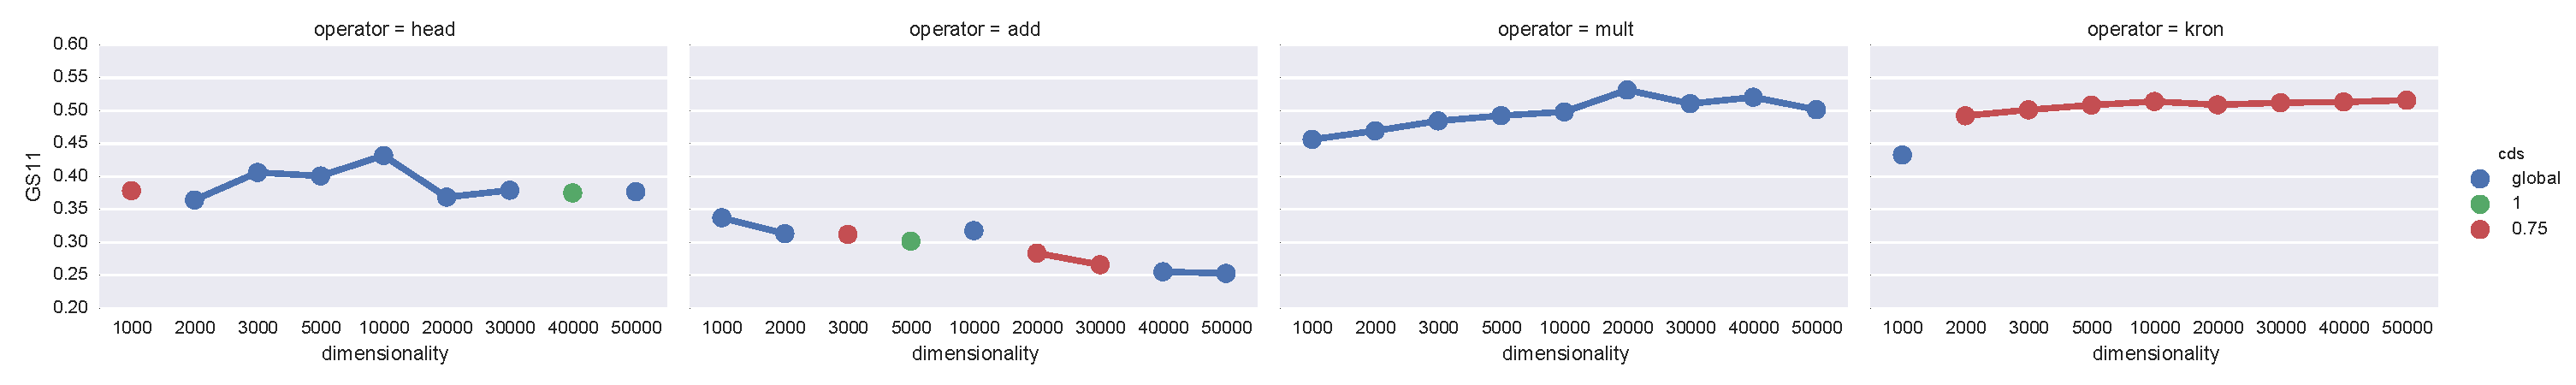
\includegraphics[width=\textwidth]{supplement/figures/GS11-max_-selection-cds}
    \caption{Max. CDS.}
    \label{fig:}
  \end{subfigure}
  % \begin{subfigure}[t]{0.7\textwidth}
  %   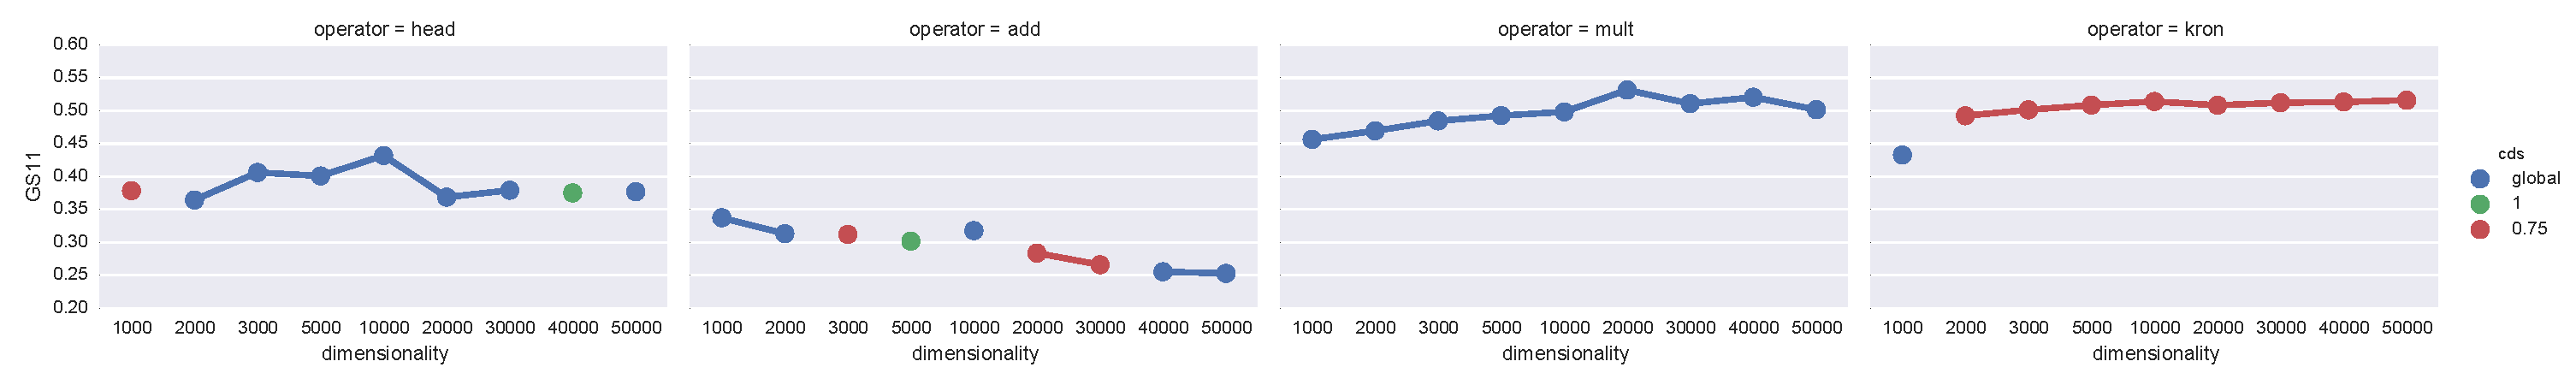
\includegraphics[width=\textwidth]{supplement/figures/GS11-cross_validation-selection-cds}
  %   \caption{CV. CDS.}
  %   \label{fig:}
  % \end{subfigure}
  \begin{subfigure}[t]{0.7\textwidth}
    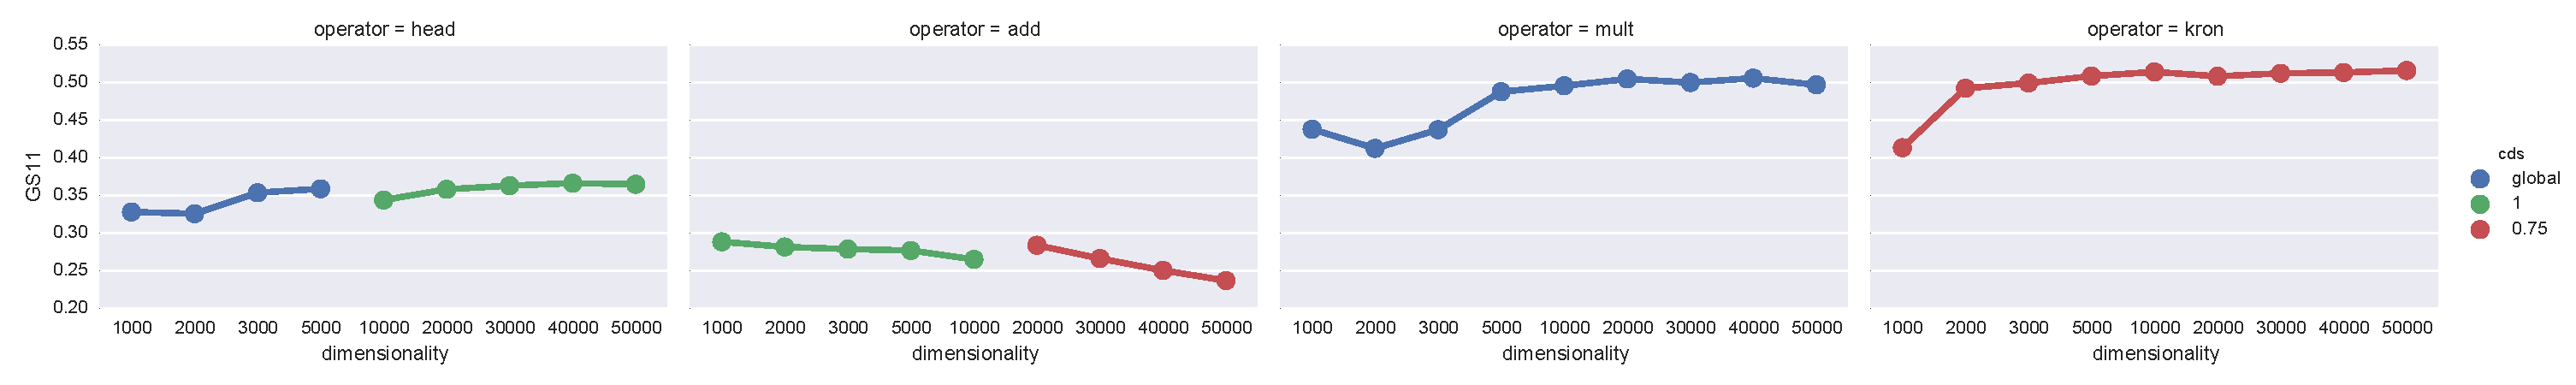
\includegraphics[width=\textwidth]{supplement/figures/GS11-heuristics-selection-cds}
    \caption{H. CDS.}
    \label{fig:}
  \end{subfigure}

  \begin{subfigure}[t]{0.7\textwidth}
    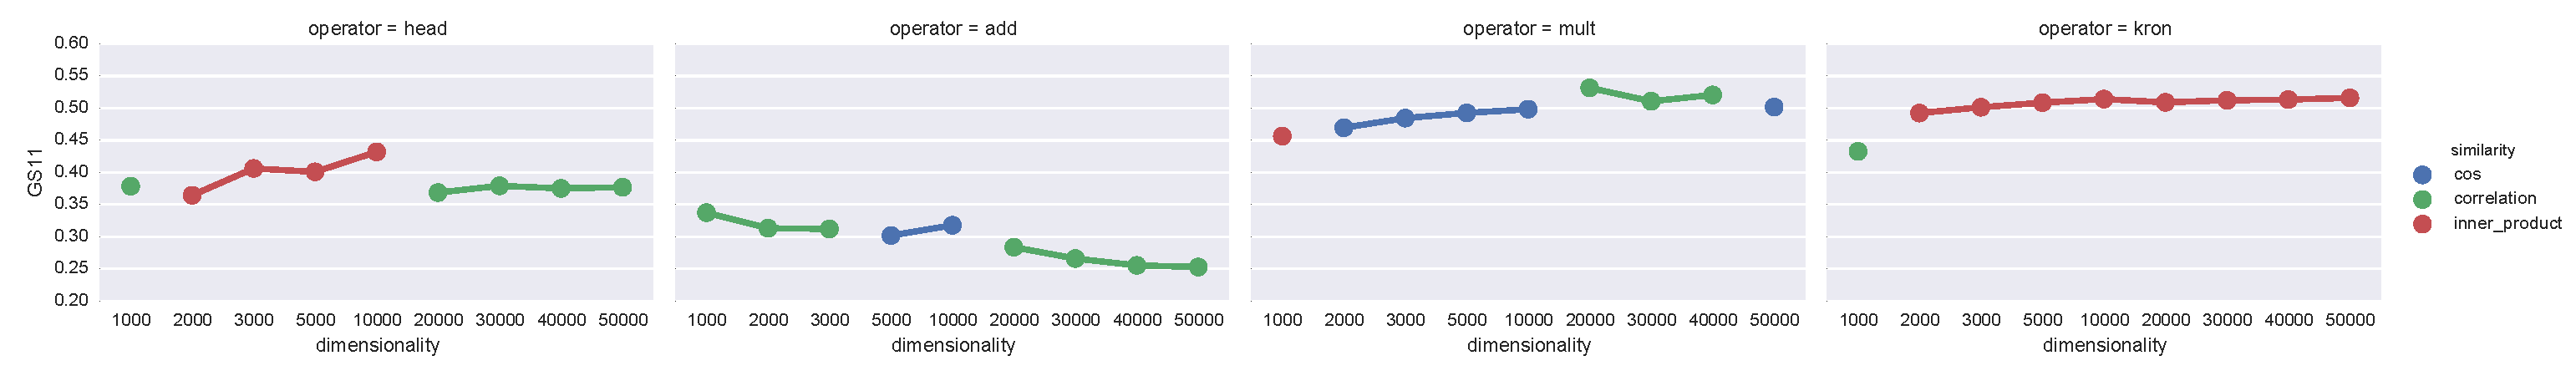
\includegraphics[width=\textwidth]{supplement/figures/GS11-max_-selection-similarity}
    \caption{Max. Sim.}
    \label{fig:}
  \end{subfigure}
  % \begin{subfigure}[t]{0.7\textwidth}
  %   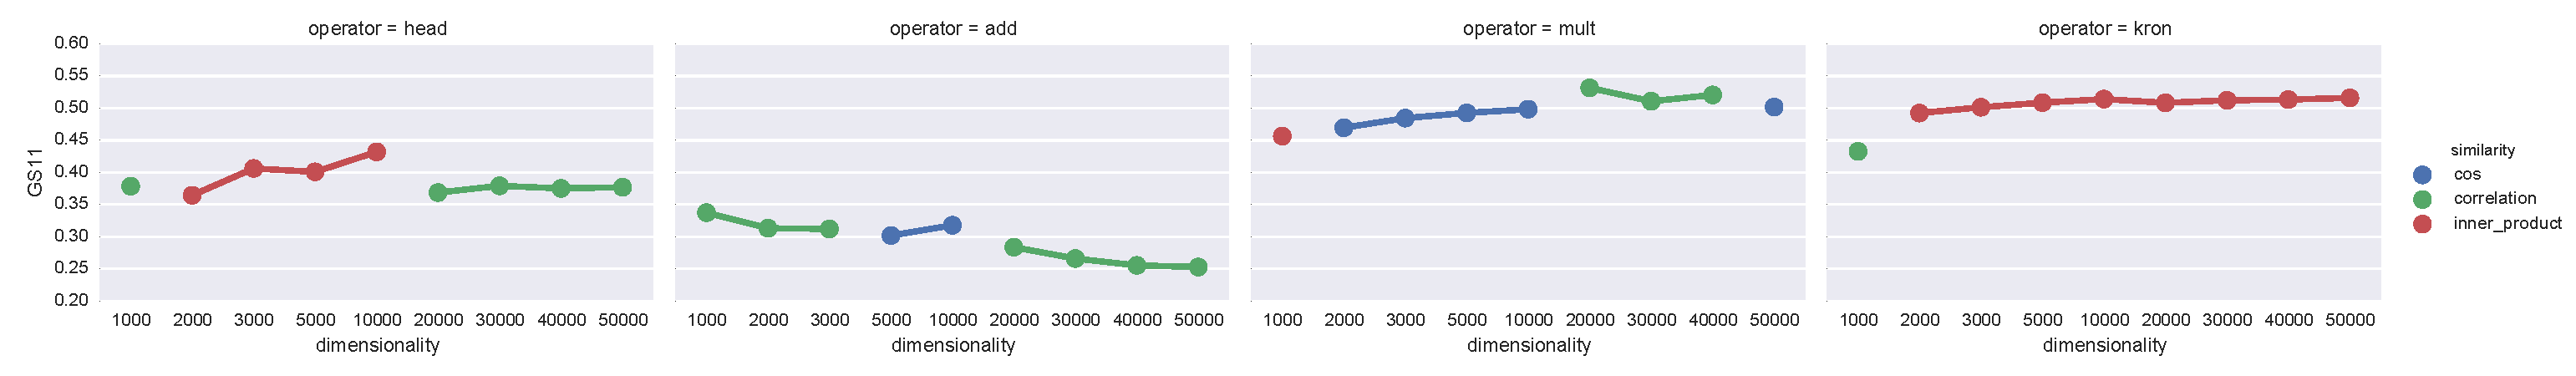
\includegraphics[width=\textwidth]{supplement/figures/GS11-cross_validation-selection-similarity}
  %   \caption{CV. Sim.}
  %   \label{fig:}
  % \end{subfigure}
  \begin{subfigure}[t]{0.7\textwidth}
    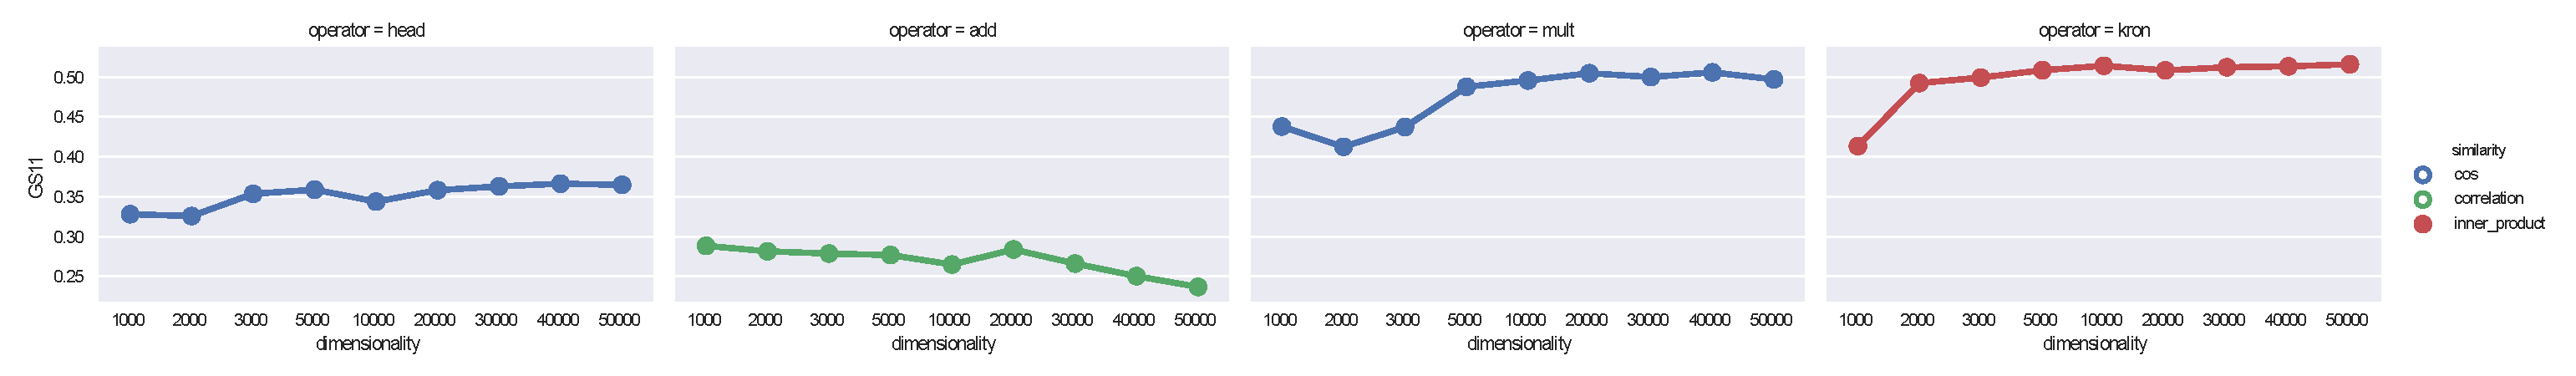
\includegraphics[width=\textwidth]{supplement/figures/GS11-heuristics-selection-similarity}
    \caption{H. Sim.}
    \label{fig:}
  \end{subfigure}

  \begin{subfigure}[t]{0.7\textwidth}
    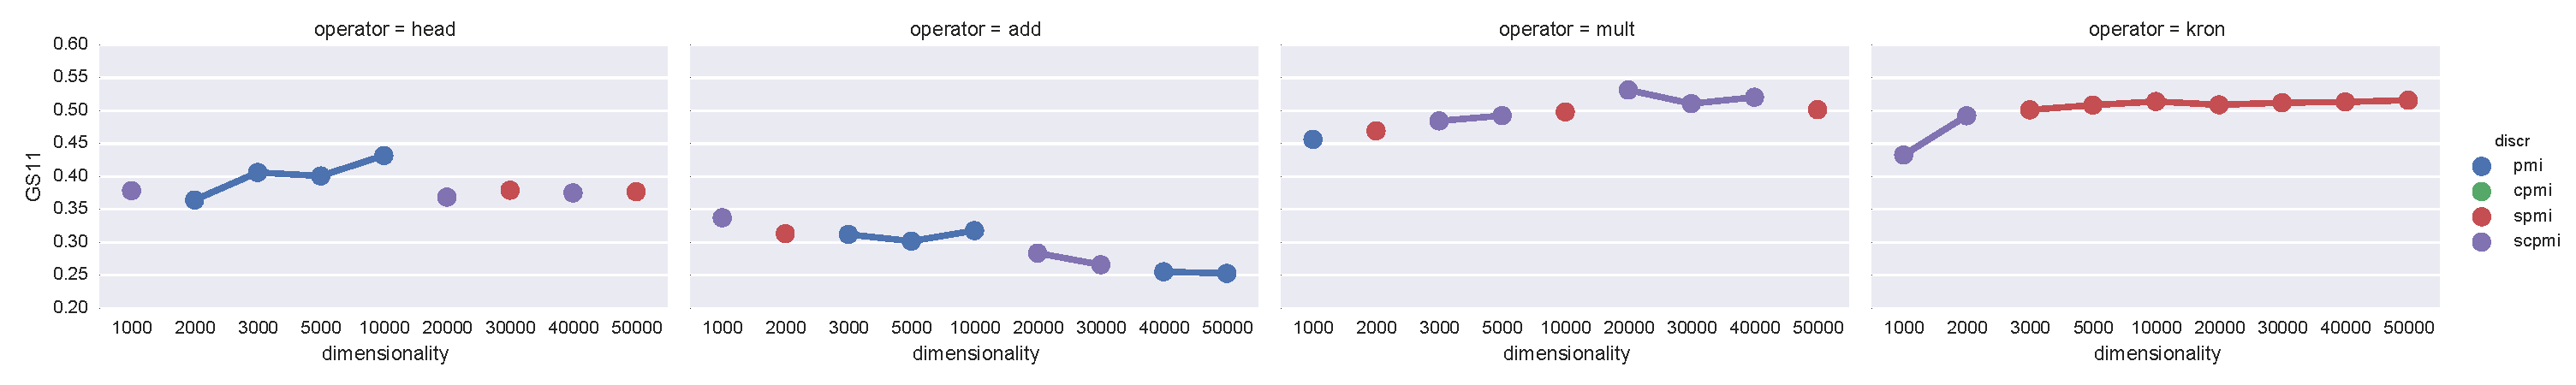
\includegraphics[width=\textwidth]{supplement/figures/GS11-max_-selection-discr}
    \caption{Max. Discr.}
    \label{fig:}
  \end{subfigure}
  % \begin{subfigure}[t]{0.7\textwidth}
  %   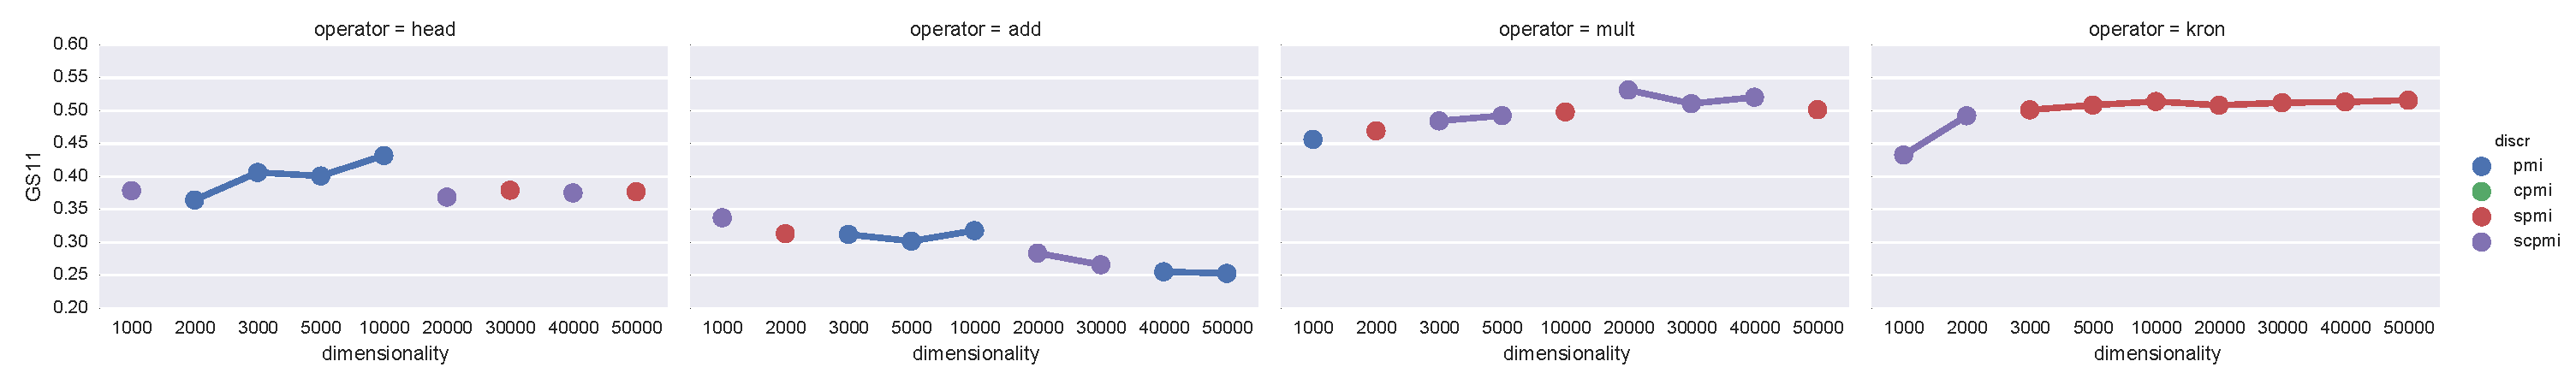
\includegraphics[width=\textwidth]{supplement/figures/GS11-cross_validation-selection-discr}
  %   \caption{CV. Discr.}
  %   \label{fig:}
  % \end{subfigure}
  \begin{subfigure}[t]{0.7\textwidth}
    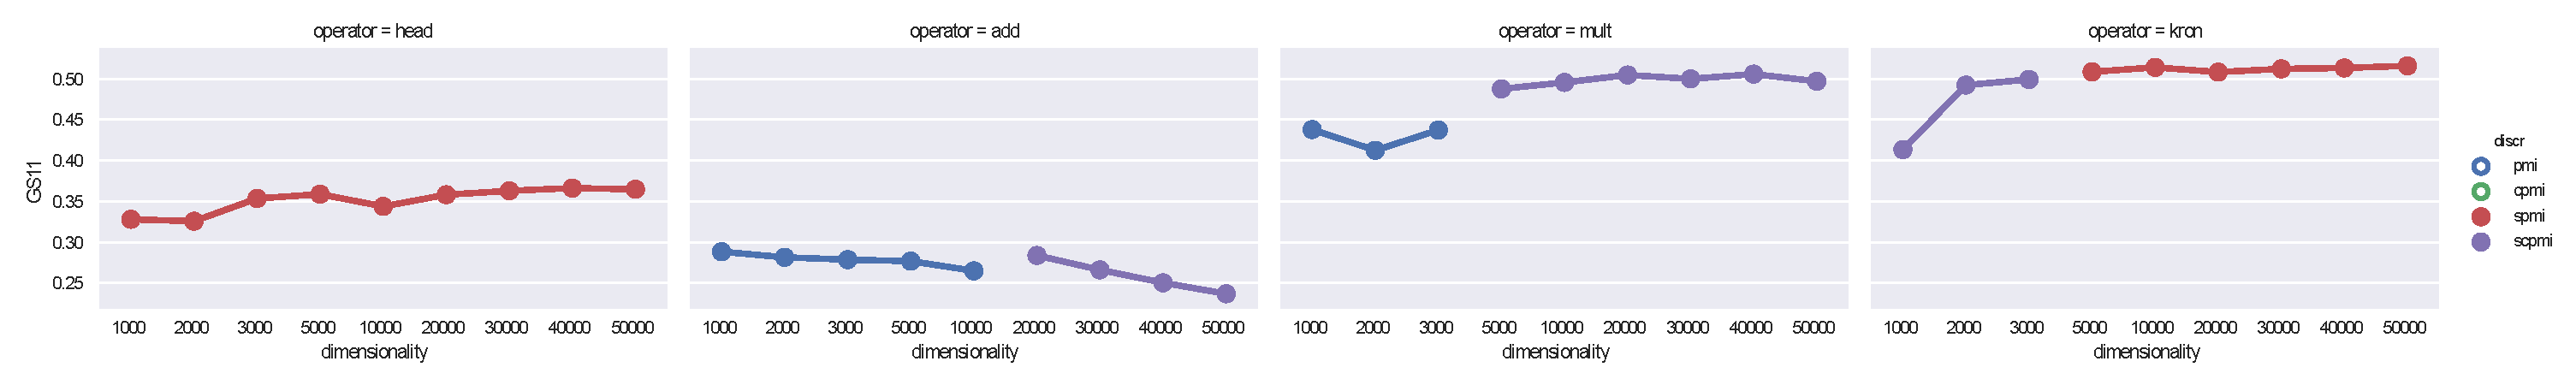
\includegraphics[width=\textwidth]{supplement/figures/GS11-heuristics-selection-discr}
    \caption{H. Discr.}
    \label{fig:}
  \end{subfigure}

  \caption{GS11 selection.}
  \label{fig:selection_gs11}
\end{figure}

\end{landscape}

\restoregeometry

% \clearpage
% \KOMAoptions{paper=A4,pagesize}
% \recalctypearea


% \subsection{MEN}
% \label{sec:men}

% \subsection{SimLex-999}
% \label{sec:simlex-999}

% \section{Similarity of sentences}
% \label{sec:sentential}

% \subsection{GS11}
% \label{sec:gs11}

% \subsection{GS12}
% \label{sec:gs12}

% \subsection{KS14}
% \label{sec:ks14}

% \subsubsection{Tweaked IR evaluation}
% \label{sec:tweak-ir-eval}

% \todo[inline]{Discuss \cite{Milajevs:2015:IMN:2808194.2809448} and link to \ref{sec:phraserel}}

% \section{PhraseRel: relevance of sentences}
% \label{sec:sentential-relevance}

%%% Local Variables:
%%% mode: latex
%%% TeX-master: "thesis"
%%% End:
